% Chapter Template

\chapter{System capabilities evaluation} % Main chapter title

\label{Chapter5} % Change X to a consecutive number; for referencing this chapter elsewhere, use \ref{ChapterX}

\lhead{Chapter 5. \emph{System capabilities evaluation}} 

\section{Indriya: Sensible, intuitive and first of its kind}
\begin{figure}
\centering
\begin{subfigure}[t]{0.49\textwidth}
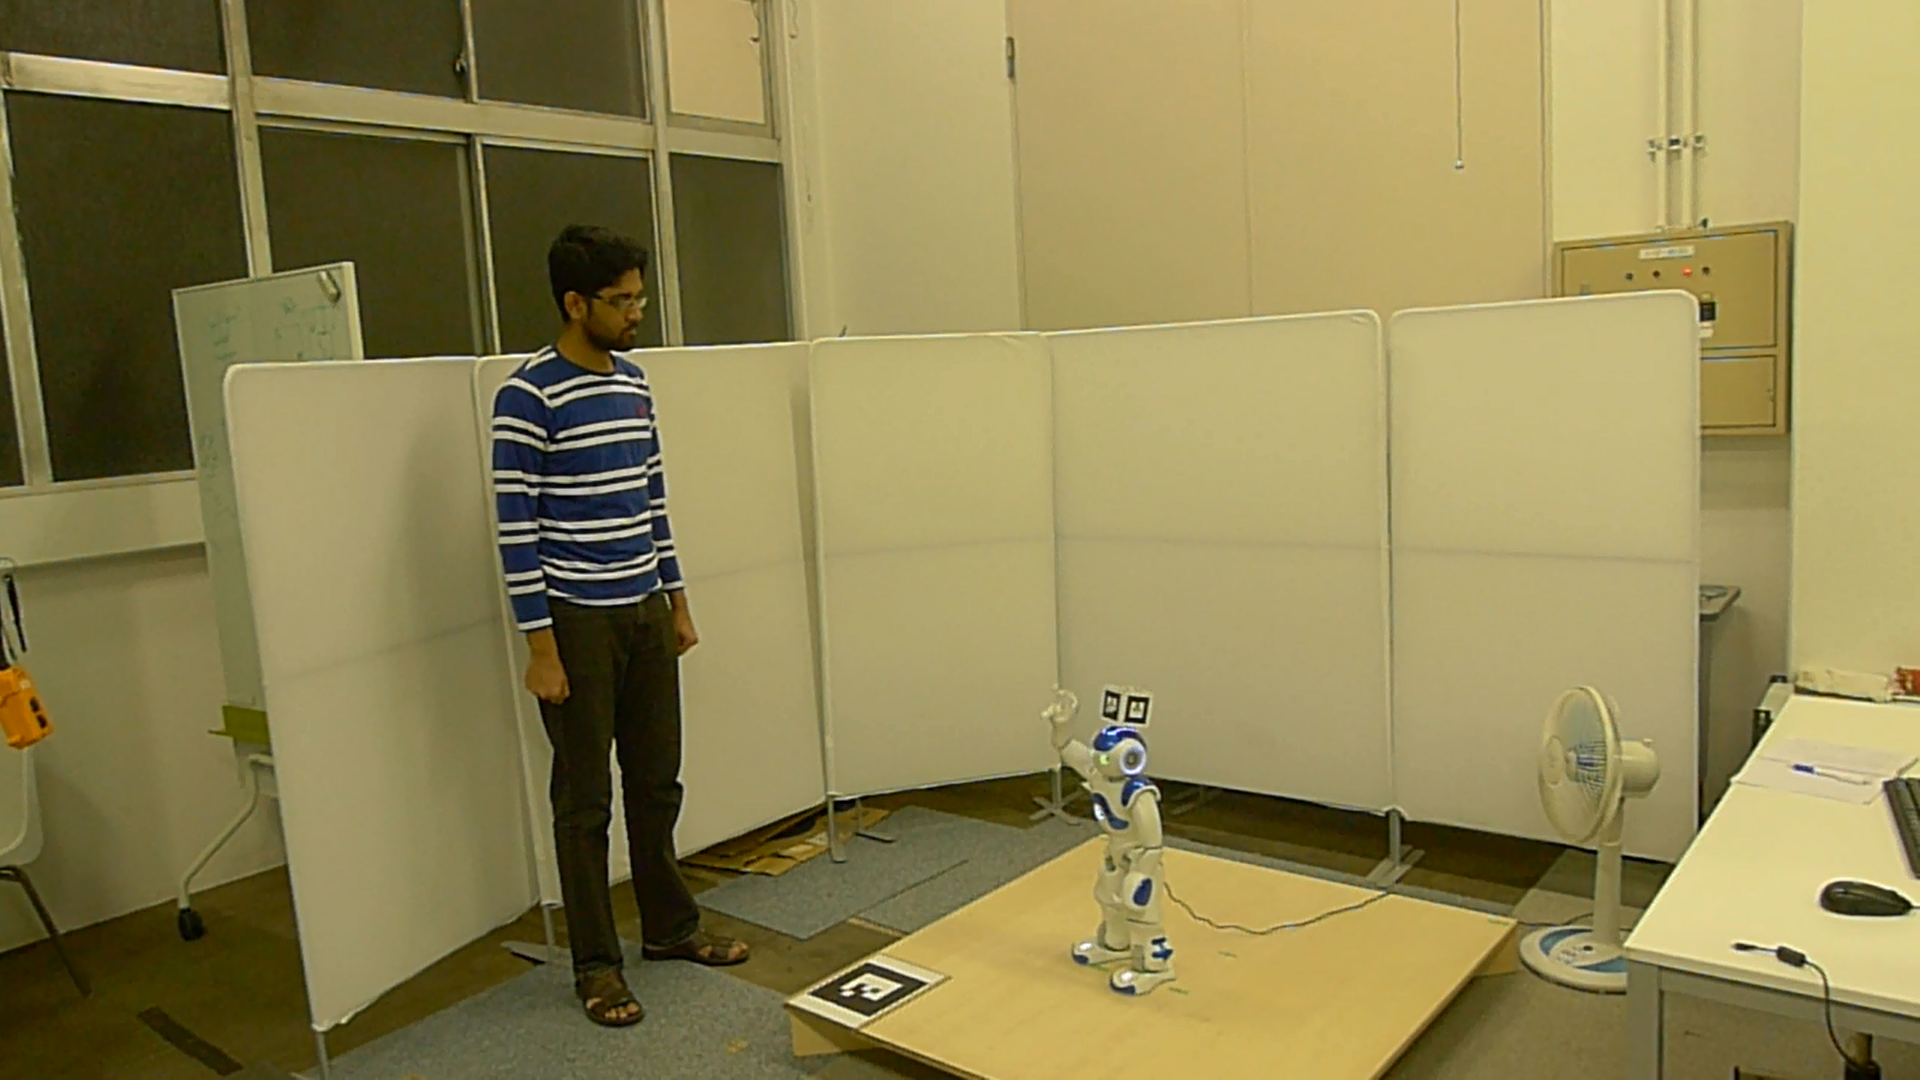
\includegraphics[width=\textwidth]{../thesis/assets/scenario_museum.png}
\caption[Experiment Setup 1]{NAO as museum guide}
\label{fig:scenario1_setup}
\end{subfigure}
\begin{subfigure}[t]{0.49\textwidth}
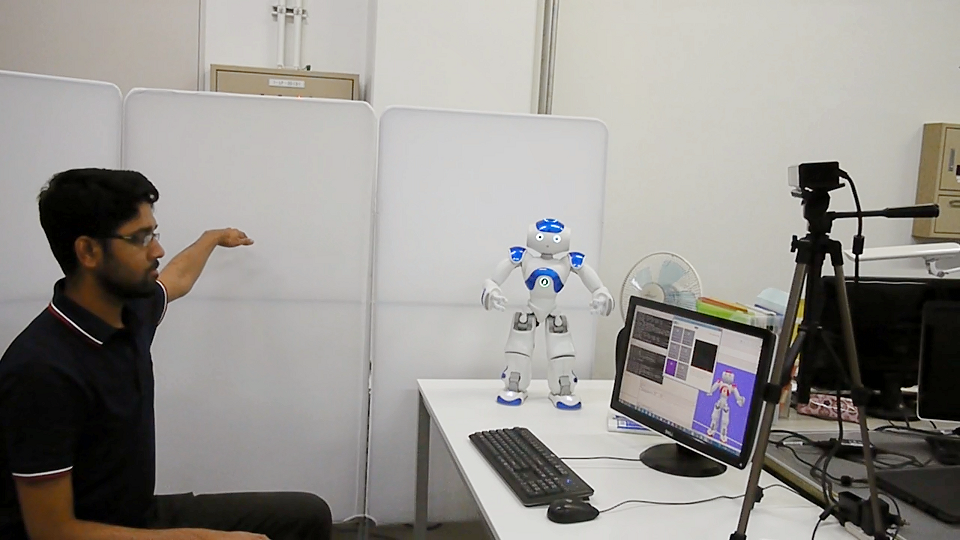
\includegraphics[width=\textwidth]{../thesis/assets/scenario_therapy.png}
\caption[Experiment Setup 2]{NAO as therapy facilitator}
\label{fig:scenario2_setup}
\end{subfigure}
\caption[Experiment Setup]{Experiment Setup}
\label{fig:scenarios_setup}
\end{figure}
	In this section we describe two scenarios to demonstrate how our behavior design system could be used for realistic cases which would be otherwise extremely difficult to realize using existing methods for a novice programmer.
\subsubsection{NAO as museum guide: }
\begin{figure}
\centering
\begin{subfigure}[t]{0.49\textwidth}
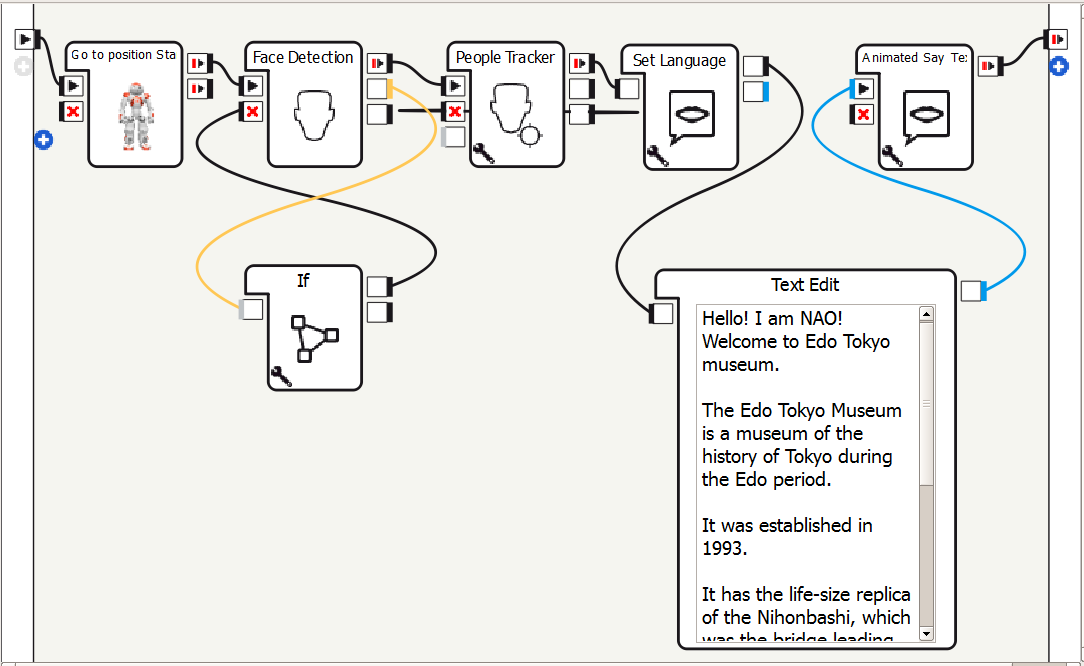
\includegraphics[width=\textwidth]{../thesis/assets/scenario_museum_choregraphe2.png}
\caption[Using Choregraphe]{Using Choregraphe}
\label{fig:scenario1_program_choregraphe}
\end{subfigure}
\begin{subfigure}[t]{0.49\textwidth}
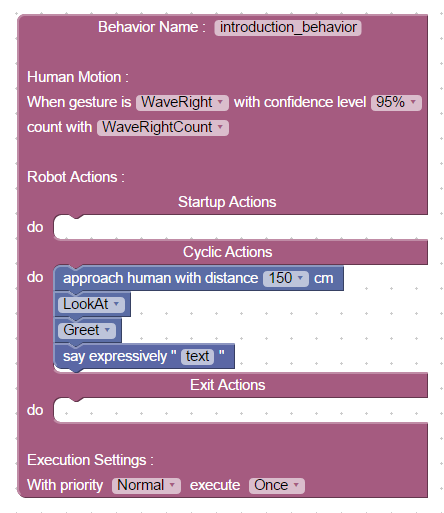
\includegraphics[width=\textwidth]{../thesis/assets/scenario1.png}
\caption[Using our behavior interface]{Using our behavior interface}
\label{fig:scenario1_program}
\end{subfigure}
\caption[NAO as museum guide]{NAO as museum guide}
\label{fig:scenarios}
\end{figure}
	The NAO humanoid robot is a guide in a museum. The museum manager would like to design a scenario where when a visitor comes into the vicinity of the robot, the robot would approach him/her and start explaining the history of the museum. We would like to use this scenario to compare the expressiveness and intuitiveness of behavior description with Choregraphe \cite{NaoRobot} shown in Fig~\ref{fig:scenario1_program_choregraphe} and with our interface shown in Fig~\ref{fig:scenario1_program}.
	
	Though Choregraphe uses a familiar flow-chart based programming model and has a huge library of primitive blocks to build complex motion patterns, the data flow for this scenario is not straight forward. As could be noticed from Fig~\ref{fig:scenario1_program_choregraphe}, at first the robot keeps looking for people in its vicinity at the cost of its power. Once it detects a person, it stops looking for people and start approaching (tracking) the person until a fixed distance with the person is reached. After this the tracking block has to be stopped and now the robot will actually start explaining the history of the museum.
	
	Using our behavior interface, the definition of this scenario is straightforward as shown in Fig~\ref{fig:scenario1_program}. The framework equipped with Kinect sensor takes care of the detection of people and gives the relative localization of the robot and human. Once the person is detected or a configured gesture trigger arrives, the behavior program retrieves the dynamic position of the robot and of the human. Using this information, the robot is driven towards the person. After coming into the proximity of the person, the robot starts explaining the history of museum. From the user perspective, the design of the behavior is intuitive and he/she can just focus on the scenario rather than thinking about the details of the data flow. The experiment setup for this scenario is shown in Fig~\ref{fig:scenario1_setup}.
\subsubsection{NAO as therapy facilitator:}%
\begin{figure}
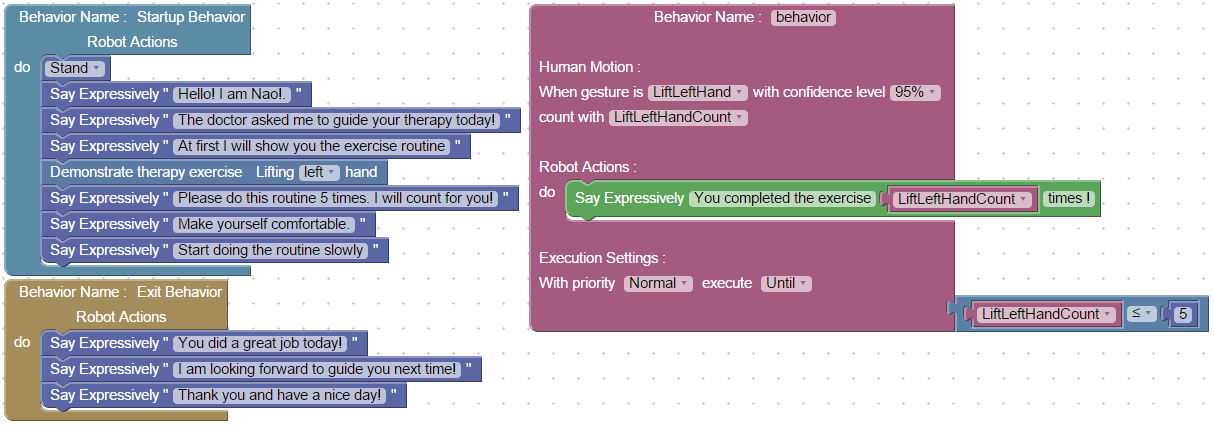
\includegraphics[width=\textwidth]{../thesis/assets/scenario2_horizontal.png}
\caption[NAO as therapy facilitator]{NAO as therapy facilitator}
\label{fig:scenario2_program}
\end{figure}
A physiotherapist who is in a remote hospital would like to prepare an exercise routine for his patient who is recovering from the fracture of his left hand. The therapist wants the service robot in the rehabilitation center to give directions to the patient in an interactive manner and facilitate the process. The exercise is composed of: an introduction and demonstration of the routine, interactively reporting the progress of the exercise and finally notifying the completion. 
	
This scenario cannot be realized using Choregraphe since it does not explicitly take into account the motion recognition. A reference implementation of such a scenario using our behavior interface is shown in Fig~\ref{fig:scenario2_program}. In the startup behavior an introduction about the exercise routine and a demonstration of the same is performed by the robot. Then each time the patient performs the exercise, the robot notifies the progress of the exercise by announcing how many times the patient has completed the exercise. Once the exercise routine is completed (say lifting left hand 5 times), the robot gives some closing comments about the routine. The experiment setup for this scenario is shown in Fig~\ref{fig:scenario2_setup}. The experiment result of the scenarios are uploaded to \url{http://youtu.be/gdbR199ejrg}

\section{Realistic scenario design}


\section{Multi-robot programming at finger tips}
Speak about the supported robots. Re usability of single module for multiple instances of same robot

\section{Parallel programming: Easier than ever before}
Collaborative introduction of Indriya system (2 Nao robots, 3 robots including turtlebot). 

\section{Priority execution making real sense}
Emergency stop scenario

\section{Summary and Discussion}

Speak about extensiblilty, modularity and software design